\documentclass[11pt,a4paper]{article}
\usepackage[latin5]{inputenc}
\usepackage[english]{babel}
\usepackage{amsmath}
\usepackage{amsfonts}
\usepackage{amssymb}
\usepackage{graphicx,subfig}
\usepackage{placeins}
\usepackage{gensymb}

\author{Alexander Attinger, Yannic Kilcher}
\title{Report Blatt 6}

\begin{document}
\maketitle

\section{Excecise 1}
\paragraph{1a}
We were asked to use a Harris Edge Detector to locate key points in the images. We tried this, but as in sheet five already noted, the Harris Detector does not seem to work very well together with a SURF Feature Matcher. Therefore we decided to use a SURF Detector instead of the Harris Detector. The resulting keypoints and the good matches are shown in Figure \ref{fig:1a}.
\paragraph{1b}
With the matches obtained in 1a, two algorithms to find the fundamental matrix $F$ were employed. Generally, given a set of matched points $(x_{i},x'_{})$ following has to hold for $F$:
\begin{equation}
x'^{T}*F*x=0 \quad \forall x
\label{eq:1}
\end{equation}
OpenCV provides the function findFundamentalMat, that given a set of matched points and will calculate $F$ using a specified algorithms. The resulting $F$ are shown below. They are similar, but not identical.

\[
\begin{array}{lc}
F_{8-point} = & \left(\begin{array}{@{}ccc@{}}
                    -9.27 & -4.45 & 0.006 \\
                    5.31 & 3.47 & 0.09 \\
                    -0.008 & -0.09 & 1
                  \end{array}\right) \\[15pt]
  
\end{array} 
\]

\[
\begin{array}{lc}
F_{RANSAC} = & \left(\begin{array}{@{}ccc@{}}
                    -1.01 & -5.01 & 0.012 \\
                    5.76 & 6.48 & 0.032 \\
                    -0.014 & -0.036 & 1
                  \end{array}\right)\\ [15pt]
  
\end{array} 
\]

The 8-Point Algorithm will take all provided points into account and try to find a solution for $F$ which will be optimal regarding the least-squares error. The RANSAC algorithm, on the other hand,differentiate between inliers and outliers and won't take outliers into accout for calculations. This can indirectly be observed by checking \ref{eq:1} for consitency. Doing this for all matches results in values relatively close to $0$ for all x, but for the points considered outliers, it is still close to $0$, but larger than for the other points (Data not shown).

\paragraph{1c}
Usually, RANSAC only considers 2-3 points as outliers. This could indicate that the key point detection and matching works quite accurate.
\begin{figure}
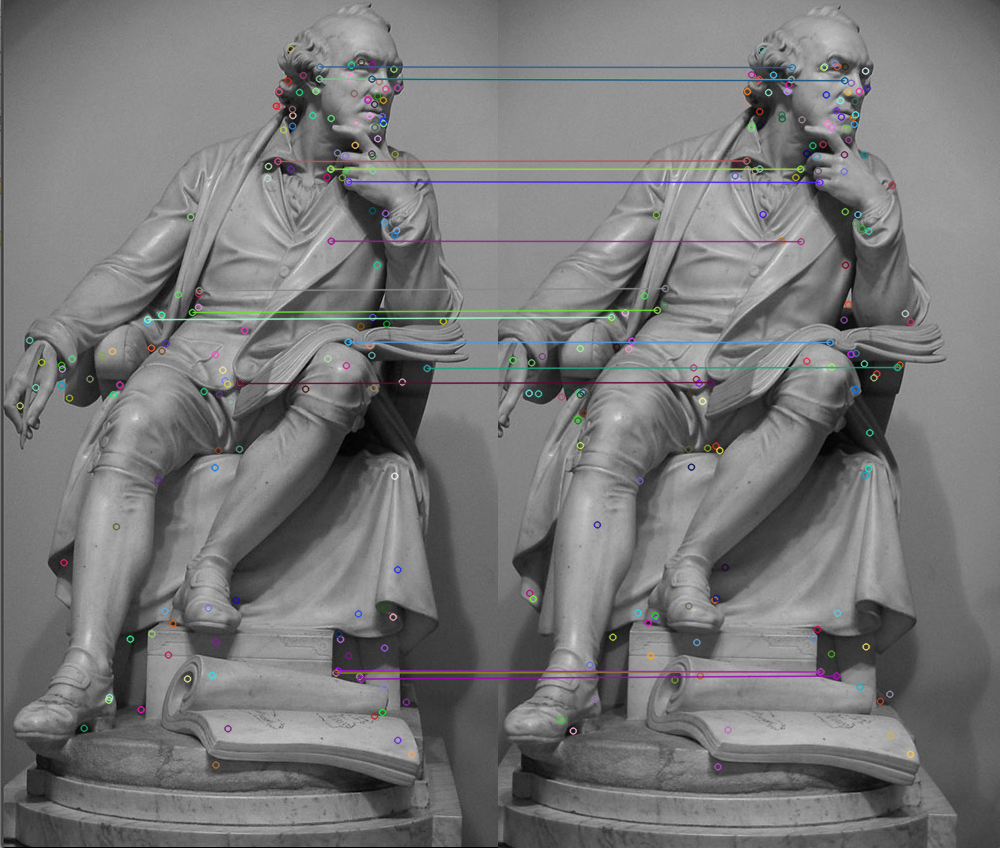
\includegraphics[scale=.4]{img/matches.png}
\caption{The two views of the John Hunter Statue with keypoints found and matched by the Surf Feature Detector and a Surf Point Matcher.}
\label{fig:1a}
\end{figure}

\begin{figure}
\centering
\subfloat[][View 1]{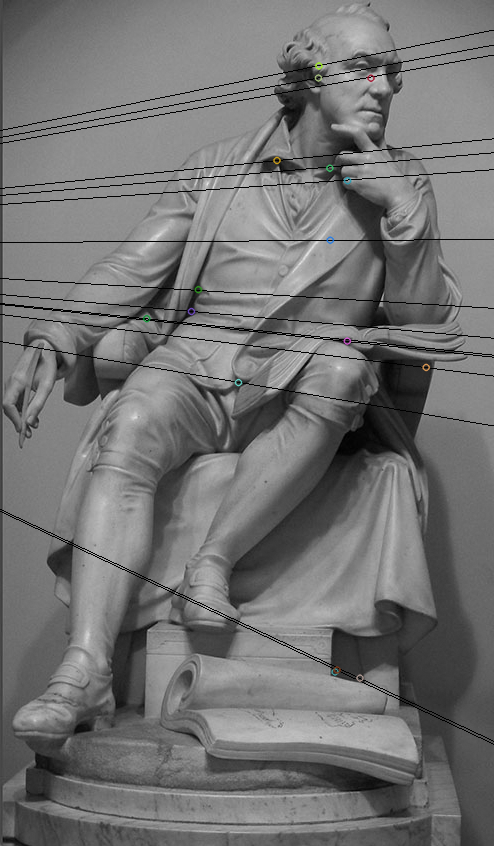
\includegraphics[scale=.3]{img/epi1.png}}
\quad
\subfloat[][View 2]{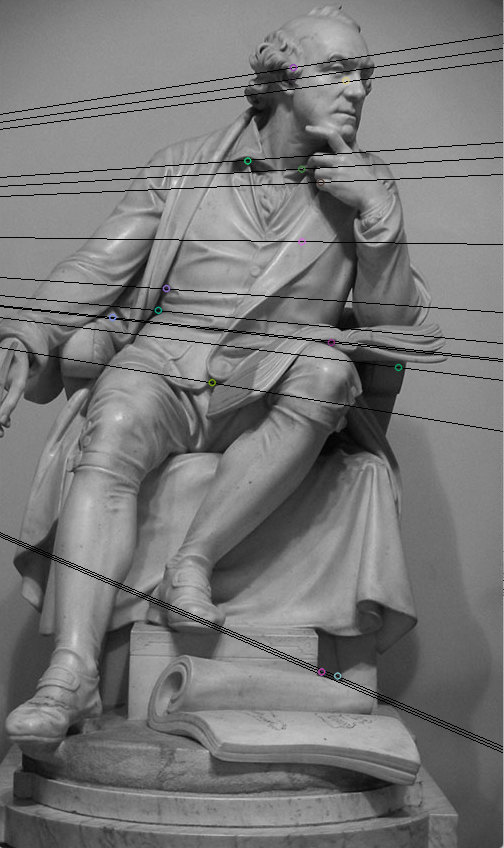
\includegraphics[scale=.3]{img/epi2.png}}

\caption{The two views of the statue. Each view contains the matched points used for the calculation of $F$. Additionally, the epipolar line for each of these points is drawn. Most of the lines pass right through the points or are right next to them, indicating a good estimate of $F$}%
\label{fig:2}
\end{figure}


\section{Excercise 2}
See Figure \ref{fig:2} for the epipolar lines. The vectors for the epipolar lines were obtained using the OpenCV function computeCorrespondEpilines, which calculates following equations:
\begin{equation}
l'_{i}=F*x_{i} \quad and \quad l_{i}=F^{T}*x'_{i}
\label{eq:2}
\end{equation}
where $l'_{i}$ is the epipolar line connecting the epipole $e'$ to $x'$ on view 2 and vice versa. Additionally, the vectors are scaled such that $l_{x}^{2}+l_{y}^{2} = 1$.
\paragraph{2b and c}
The distance $d$ between a point $x$ and its corresponding epipolar line $l$ is then given by:
\begin{equation}
d=x^{T}*l
\end{equation}
The average distance between the points and the epipolar lines in view two is $0.48$ and in view one it is $0.49$. So less than half a pixel. For inliers only, it is $0.32$ in view two and $0.33$ in view one. The average distance between point and corresponding epiline seems to be small, indicating again a good estimate for $F$ and confirming the observation in Figure \ref{fig:2}. There is a problem, however. We believe that the epipoles of one image should lie in the direction of the other image, since it has to lie on the line connecting the two camera centers. See discussion for more about this.
\paragraph{Discussion}
Following can be assumed about the scene: The statue is is probably relatively big, i.e. the pictures are taken from relatively far away. This resuts in minute perspective effects, the transformation from the world space into the image plane is almost affine. I.e. the resulting $F$ should be represent an affine transformation (all elements except last row and last column zero). This is not the case (see Excercise one). We assume that some of the errors made in the point matching are somehow 'accounted for' by creating a non affine $F$. This $f$ will satisfy \ref{eq:1} quite well and the lines obtained with \ref{eq:2} will go through connect the matched points and the epipoles well. However, the observed location of the epipoles is strange. We believe that in this situation the observed epipolar lines should be almost parallel.

When the threshold of both the SURF Point Detector and the SURF Point Matcher are made less strict, more points are taken into account to calculate F, resulting in an estimation of F which hopefully represents the real $F$ better. The fundamental Matrix obtained with the matches seen in Figure \ref{fig:3} is:
\[
\begin{array}{lc}
F_{RANSAC} = & \left(\begin{array}{@{}ccc@{}}
                    0.00 & 0.00 & -0.001 \\
                    0.00 & 0.00 & 0.099 \\
                    -0.02 & -0.10 & 1
                  \end{array}\right)\\ [15pt]
  
\end{array} 
\]

The values denoted with $0.00$ are not actually $0$, but lie in the range of $10^{-6}$. This $F$ acutally is very similar to an fundamental Matrix obtained in a purely affine situation. The epipolar lines obtained in this way are almost parallel, as can be seen in Figure \ref{fig:4}.

\begin{figure}
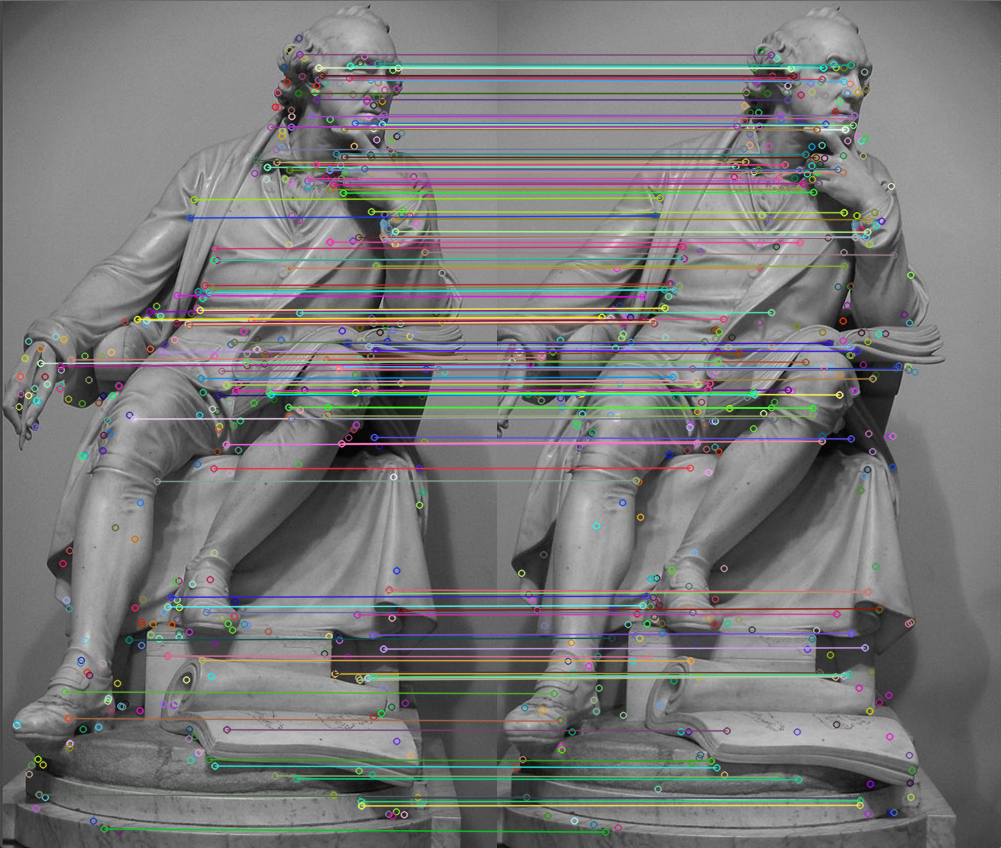
\includegraphics[scale=.4]{img/matches2.png}
\caption{The two views of the John Hunter Statue with keypoints found and matched by the Surf Feature Detector and a Surf Point Matcher. The thresholds have been chosen such that more points are detected and matched.}
\label{fig:3}
\end{figure}

\begin{figure}
\centering
\subfloat[][View 1]{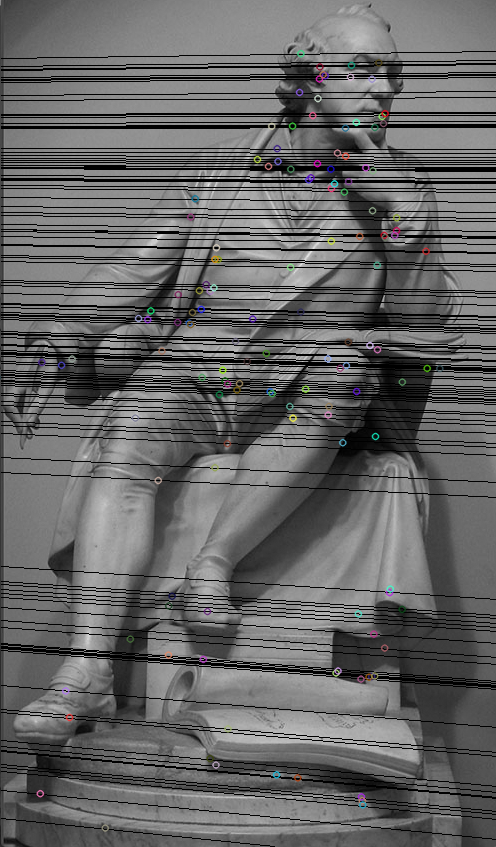
\includegraphics[scale=.3]{img/epi2_1.png}}
\quad
\subfloat[][View 2]{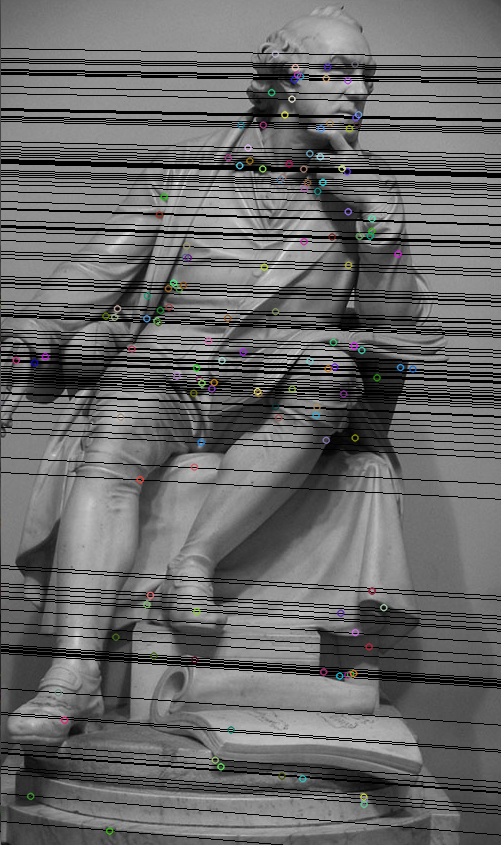
\includegraphics[scale=.3]{img/epi2_2.png}}

\caption{The two views of the statue. Each view contains the matched points used for the calculation of $F$. Additionally, the epipolar line for each of these points is drawn. Most of the lines pass right through the points or are right next to them, indicating a good estimate of $F$}%
\label{fig:4}
\end{figure}

\end{document}